%region achieved by the ENP test is a curve/ The Gaussian Case
\section{The M-ROC Surface  under Gaussian Hypotheses}
In the following we present two examples, for computing the M-ROC for Gaussian Hypotheses. 

\noindent \textbf{Example 1:}

Assume three hypotheses given as:
\begin{equation}
\label{equ: Gaussian Hypothesis}
\begin{split}
	H_0:\;\;\;\;\;\;\;\;&X \sim \mathcal{N}(-1,1)\\
    H_1:\;\;\;\;\;\;\;\;&X \sim \mathcal{N}(0,1)\\
    H_2:\;\;\;\;\;\;\;\;&X \sim \mathcal{N}(1,10)\,,
\end{split}
\end{equation}
where $\mathcal{N}(\mu,\sigma^2)$ denotes a Gaussian PDF with mean $\mu$ and variance $\sigma^2$.
To form the M-ROC surface, we first consider points that belong to $M_0$.
From section 3.1, we can see that when $(P_d, c_1, c_2) \in M_0$, there exists non-negative $\mathbf{k}$ such that by using decision rule 
\begin{equation}
f_0(x) \substack{H_0 \\ \geq \\ < \\ \bar{H}_0} k_1f_1(x) + k_2f_2(x)
\end{equation}
we have 
\begin{equation}
\begin{split}
\label{1125c0}
&P_d = \int_{-\infty}^{\infty} u(f_0(x) - \sum_{j=1}^{2}k_jf_j(x)) f_0(x)\mathrm{d}x    \,, \\
&P_{f_i} = \int_{-\infty}^{\infty} u(f_0(x) - \sum_{j=1}^{2}k_jf_j(x)) f_i(x) \mathrm{d}x = c_i\;\;\;\;\;    i=1, 2\,.
\end{split}
\end{equation}
We use Matlab to compute the M-ROC for region $M_0$. The values of $k_1$ and $k_2$ range from $0$ to $100$ in steps of $0.01$. Substituting the value of $k_1$ and $k_2$ into \eqref{1125c0}, results in the corresponding $P_d$ $P_{f_1}$ and $P_{f_2}$.  The set $M_0$ is illustrated in Figure \ref{pic: surface for m0 gaussian}. 
From the definition of $M_0$, we know its projection on the $c_1-c_2$ plane is $\alpha^+$.  
 The set $\alpha^+$ for this example is presented in Figure \ref{pic: contour for m0 gaussian}. 

\begin{figure}[!t]
\centering
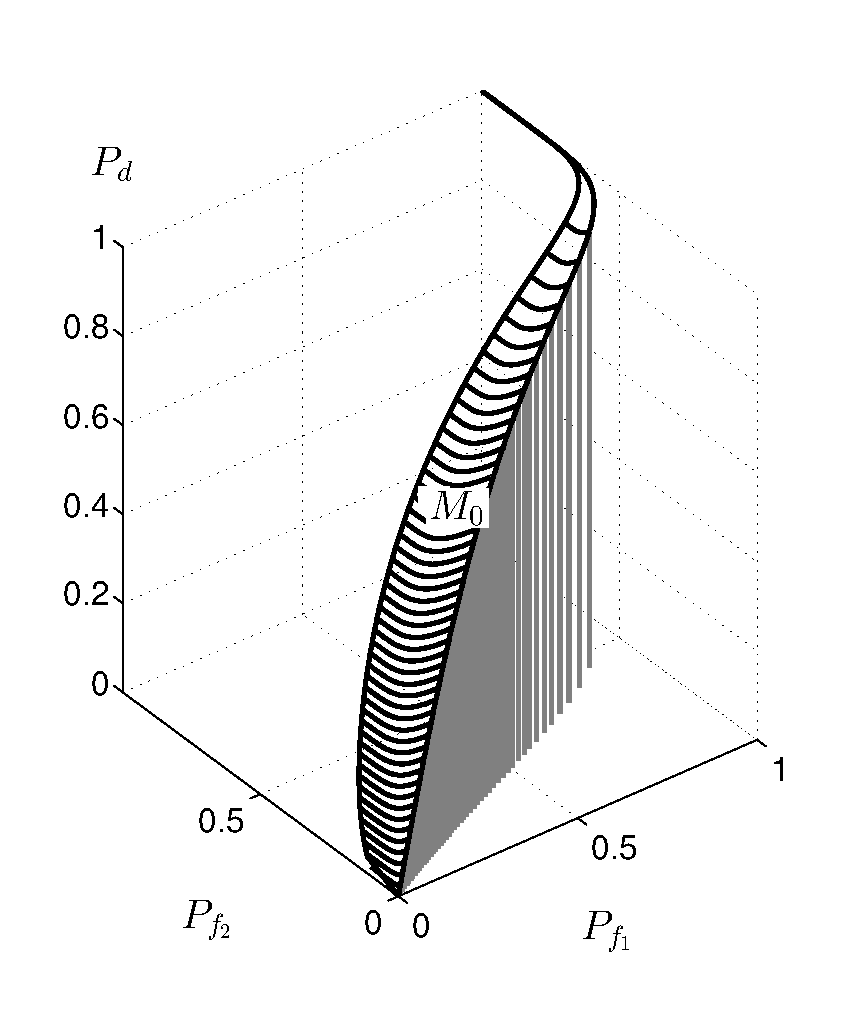
\includegraphics[width=12cm, height=16cm]{3/singleROC.eps}
\caption{Region that can be achieved by Neyman Pearson testing with $k_i \geq 0 (i=1, ..., M)$.}
\label{pic: surface for m0 gaussian}
\end{figure}

\begin{figure}[!t]
\centering
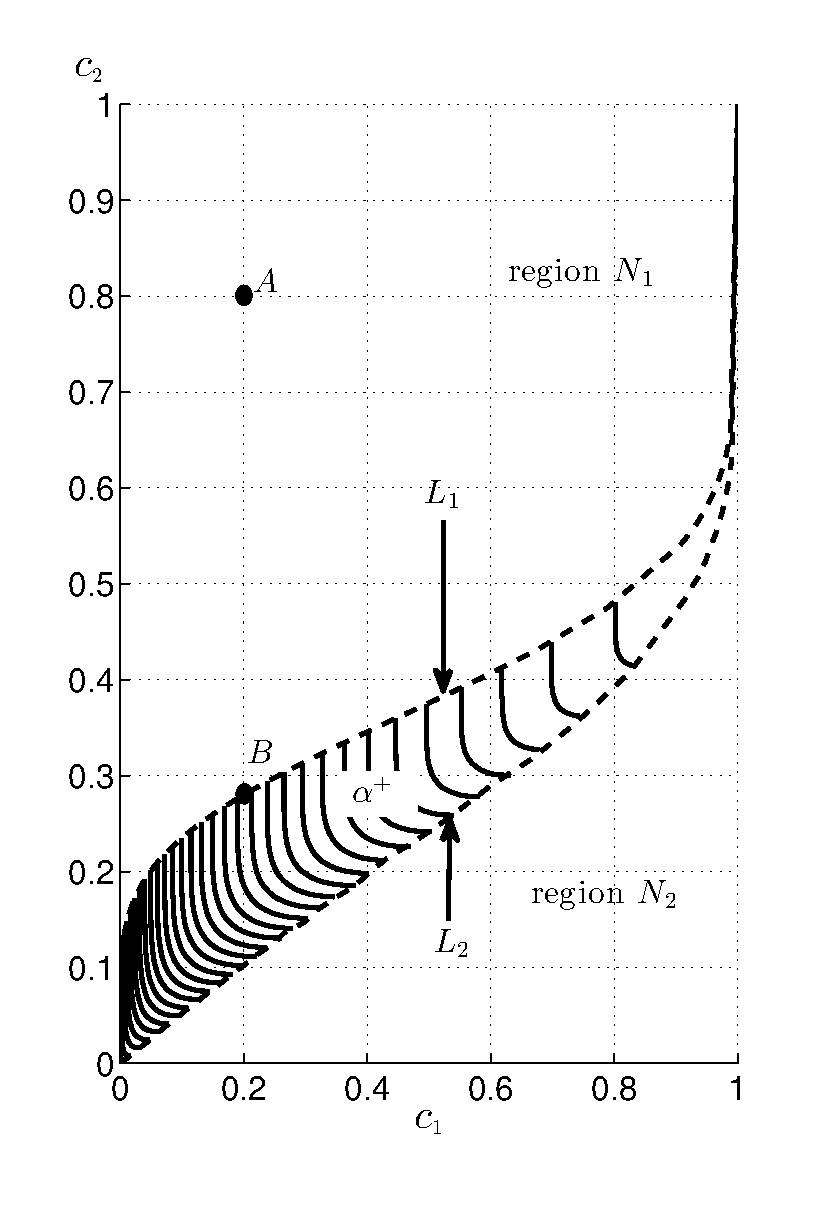
\includegraphics[width=12cm, height = 16cm]{3/singlecontour.eps}
\caption{Region that can be achieved by Neyman Pearson testing with $k_i \geq 0 (i=1, ..., M)$.}
\label{pic: contour for m0 gaussian}
\end{figure}

\begin{figure}[!t]
\centering
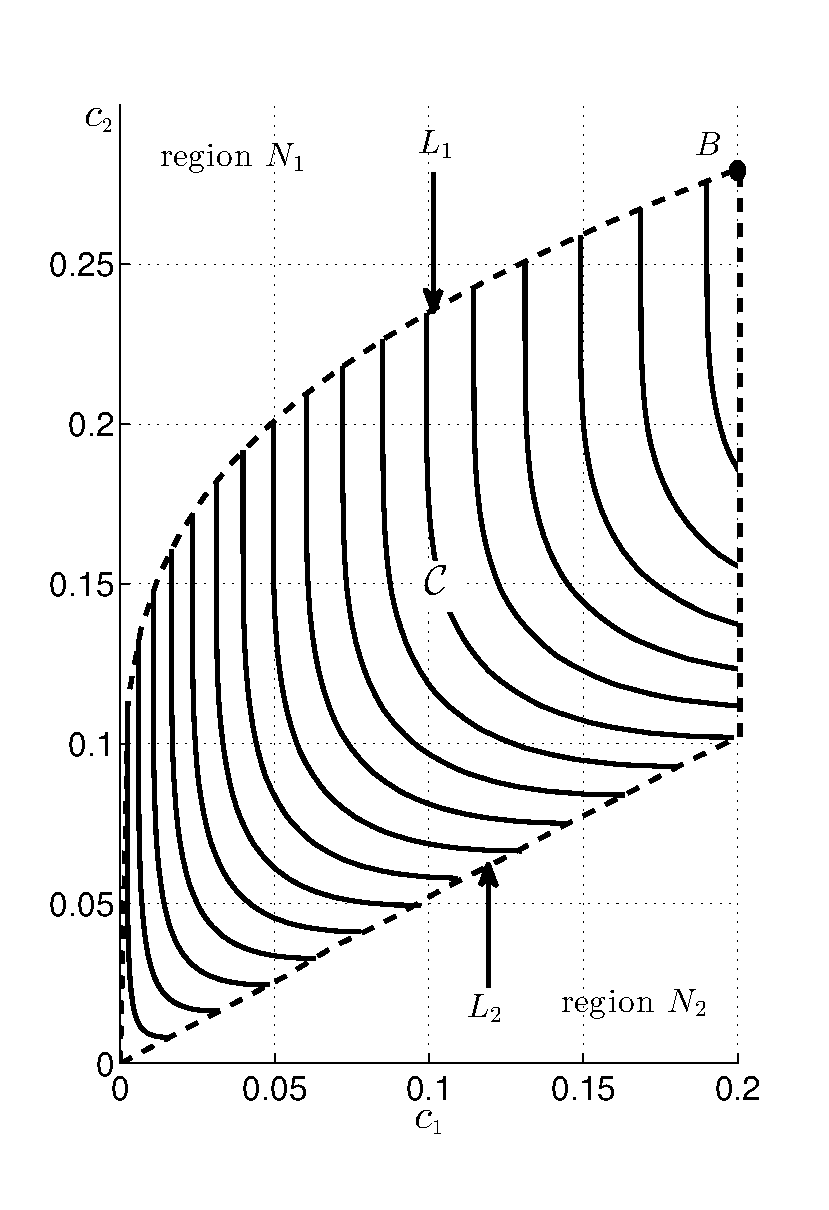
\includegraphics[width=12cm, height = 16cm]{3/singlecontour2.eps}
\caption{The region $\mathcal{C}$ when $c_1 = 0.2$ and $c_2 = 0.8$.}
\label{pic: regionC}
\end{figure}

Define curve $L_1$ as the set of points 
\[
\{ (c_1, c_2) \in L_1 | (c_1, c_2) \in \alpha^+ \;\;\text{and} \;\;(c_1, c_2+\epsilon)\notin \alpha^+ \;\;\;\;\text{for any positive $\epsilon$} \}\,.
\]
Define curve $L_2$ as the set of points 

\[
\{ (c_1, c_2) \in L_2 | (c_1, c_2) \in \alpha^+ \;\;\text{and} \;\;(c_1 + \epsilon, c_2)\notin \alpha^+ \;\;\;\;\text{for any positive $\epsilon$} \}\,.
\]
Let $N_1$ denote the region enclosed by line $c_1 = 0$, $c_2$; line $c_1$, $c_2 = 1$ and curve $L_1$.
Let $N_2$ denote the region enclosed by line $c_1 = 1$, $c_2$; line $c_1$, $c_2 = 0$ and curve $L_2$.
The regions $\alpha^+$, $N_1$ and $N_2$ are shown in Figure \ref{pic: contour for m0 gaussian}.

In the following, we present the decision rule for points belong to regions $N_1$ or $N_2$.

\noindent \textbf{Property 2:}
\textit{\\(1) All points belonging to region $N_1$ or curve $L_1$, if they have the same $c_1$, they have the same decision rule and same $P_d$.
\\(2) All points belonging to region $N_2$ or curve $L_2$, if they have the same $c_2$, they have the same decision rule and same $P_d$.
}

\noindent \textbf{PROOF}
Recall $F(\mathbf{c})$ is defined as the largest $P_d$ that can be achieved under constraint $\mathbf{P}_f = \mathbf{c}$ and 
       $G(\mathbf{c})$ is defined as the largest $P_d$ can be achieved under constraint $\mathbf{P}_f \leq \mathbf{c}$.
Firstly we will show $F(\mathbf{c}) = G(\mathbf{c}) $ when $\mathbf{c} \in \alpha^+$.

According to the definition of $\alpha^+$, for a point $(c_1, c_2) \in \alpha^+$, there exists a decision rule 
\[
\delta:\;\;\;\;f_0(x) \substack{H_0 \\ \geq \\ < \\ \bar{H}_0} k_1f_1(x) + k_2f_2(x) \;\;\;\;(k_1, k_2 \geq 0)
\]
such that under decision rule $\delta$, we have 
\begin{equation}
\label{1125a3}
\mathbf{P}_{f}(\delta) = \mathbf{c}\,.
\end{equation}
From ENP Lemma (\rmnum{2}), we know 
\begin{equation}
\label{1125c1}
P_d(\delta) = F(\mathbf{c})\,.
\end{equation}
Since $k_1, k_2 \geq 0$, according to ENP Lemma (\rmnum{3}), $\delta$ also achieve the largest $P_d$ while keeping $\mathbf{P}_f \leq \mathbf{c}$, i.e. 
\begin{equation}
 P_d(\delta) =G(\mathbf{c}) 
\label{1125a2}
\end{equation}
From \eqref{1125c1} and \eqref{1125a2} we can see $F(\mathbf{c}) = G(\mathbf{c})$ for $\mathbf{c} \in \alpha^+$.
In Section 2.2.2,  we have shown $G(\mathbf{c})$ is a non-decreasing function for each variable of $\mathbf{c}$, hence it can be concluded that $F(\mathbf{c})$ is a non-decreasing function for each variable of $\mathbf{c}$ on set $\alpha^+$.

As it is shown in Figure \ref{pic: contour for m0 gaussian}, A is a point in region ${N}_1$ with coordinates $(c_1, c_2) = (c_{1_A}, c_{2_A})$. In the following we will derive its optimal decision rule through MENP test. By optimal decision rule, we mean   it achieves the largest $P_d$ while keeping $\mathbf{P}_f \leq \mathbf{c}$.  
As point A does not belong to $\alpha^+$, we should use MNEP (\rmnum{2}) to get its decision rule. To do it, the first step is to determine set $\mathcal{C}$, which is the intersection of $\mathcal{A}_c$ and $\alpha^+$. In this case, set $\mathcal{C}$ is plotted in Figure \ref{pic: regionC}.
After we have $\mathcal{C}$, we need to find $\mathbf{c}^0 \in \mathcal{C}$ such that it maximum $F(\mathbf{c})$ among all $\mathbf{c} \in \mathcal{C}$.
Figure \ref{pic: contour for m0 gaussian} and Figure \ref{pic: regionC} shows that point B (with coordinate $(c_{1_B}, c_{2_B})$ where $c_{1_B} = c_{1_A}$) has the largest $c_1$ $c_2$ components among all $\mathbf{c} \in \mathcal{C}$. Since $F(\mathbf{c})$ is a non-decreasing function for $c_1$ and $c_2$ on set $\alpha^+$, it is easy to see
\begin{equation}
  \max_{\mathbf{c} \in \mathcal{C}}\;\;\;\;F(\mathbf{c}) = F(c_{1_B}, c_{2_B})\,.
  \label{2015apr30a0}
\end{equation}
 As point B is in set $\mathcal{C}$, there exists decision rule
 \[
\delta^\ast:\;\;\;\;f_0(x) \substack{H_0 \\ \geq \\ < \\ \bar{H}_0} k_1^\ast f_1(x) + k_2^\ast f_2(x) \;\;\;\;(k_1^\ast, k_2^\ast \geq 0)
 \]
 such that under $\delta^\ast$ we have  $P_{f_1}(\delta^\ast) = c_{1_B}$ and  $P_{f_2}(\delta^\ast) = c_{2_B}$. 
 From ENP (\rmnum{3}), it is easy to see $\delta^\ast$ is the optimal decision rule for point B.
 Since point B satisfies \eqref{2015apr30a0}, by using MENP (\rmnum{2}), we know $\delta^\ast$ is also the optimal decision rule for point A. Thus we can see the optimal decision rule for point A and point B are the same. Since point A lies in region $N_1$, point B lies in region $L_1$ and $c_{1_A} = c_{1_B}$, we can conclude for two points respectively belongs to $N_1$ and $L_1$, if they have the same $c_1$ component, they have the same decision rule and same $P_d$. 

Furthermore, we can see as long as A is in region $N_1$ its decision rule only depends on the value of $c_{1}$.  In other words, as long as A is in region $N_1$, with $c_1 = c_{1_A}$ fixed,  when $c_{2}$ changes, its optimal decision rule and $P_d$ remain the same. Hence we can conclude all points belonging to region $N_1$ or curve $L_1$, if they have the same $c_1$, they have the same decision rule and same $P_d$.

In the same way, we can prove: For points belong to region $N_2$ or curve $L_2$, if they have the same $c_2$ value, they have the same decision rule and same $P_d$.

Q.E.D

Since we have computed $P_d$ for $(c_1, c_2) \in N_0$ and curves $L_1$ and $L_2$ belong to $N_0$, we can get $P_d$ for $(c_1, c_2)$ belongs to $N_1$ or $N_2$ through \textbf{Property 2}. M-ROC surface for this example is given in Figure  \ref{pic: LJS}.
The whole M-ROC is divided into three regions ($M_1$, $M_0$ and $M_2$) to simplify our analysis.  
 The projection of $M_1$ on $c_1-c_2$ plane is set $N_1$, and the projection of $M_2$ on $c_1-c_2$ plane is set $N_2$. 
In region $M_1$, $P_d$ increases if and only if the value of $c_1$ increases, the value of $c_2$ does not affect $P_d$. On the opposite, in region $M_2$, $P_d$ increases if and only if the value of $c_1$ increases, it does not change with $c_2$. In region $M_0$, when one of $c_1$ or $c_2$ increases, $P_d$ will increase. In all these three regions, $P_d$ is non-decreasing with respect to $c_1$ and $c_2$. 

Next we discuss the different between the ENP test and MENP test concerning this example. 
From Figure \ref{pic: surface for m0 gaussian}, we can see the ENP test works only when the given $(c_1, c_2)$ belongs to set $\alpha^+$. For the case when $(c_1, c_2) \notin \alpha^+$, it cannot provide a solution.  However,  from Figure \ref{pic: LJS}, it can be seen by using the MENP test, we can get the decision rule for all $(c_1, c_2)$. 
In other words, the achievable region of the MENP test is larger than that of the ENP test. 
Besides that, we can see when $(c_1, c_2) \in \alpha^+$, the ENP test and the MENP test provides the same $P_d$. This results from the repetition between the two frameworks.  
\begin{figure}[!t]
\centering
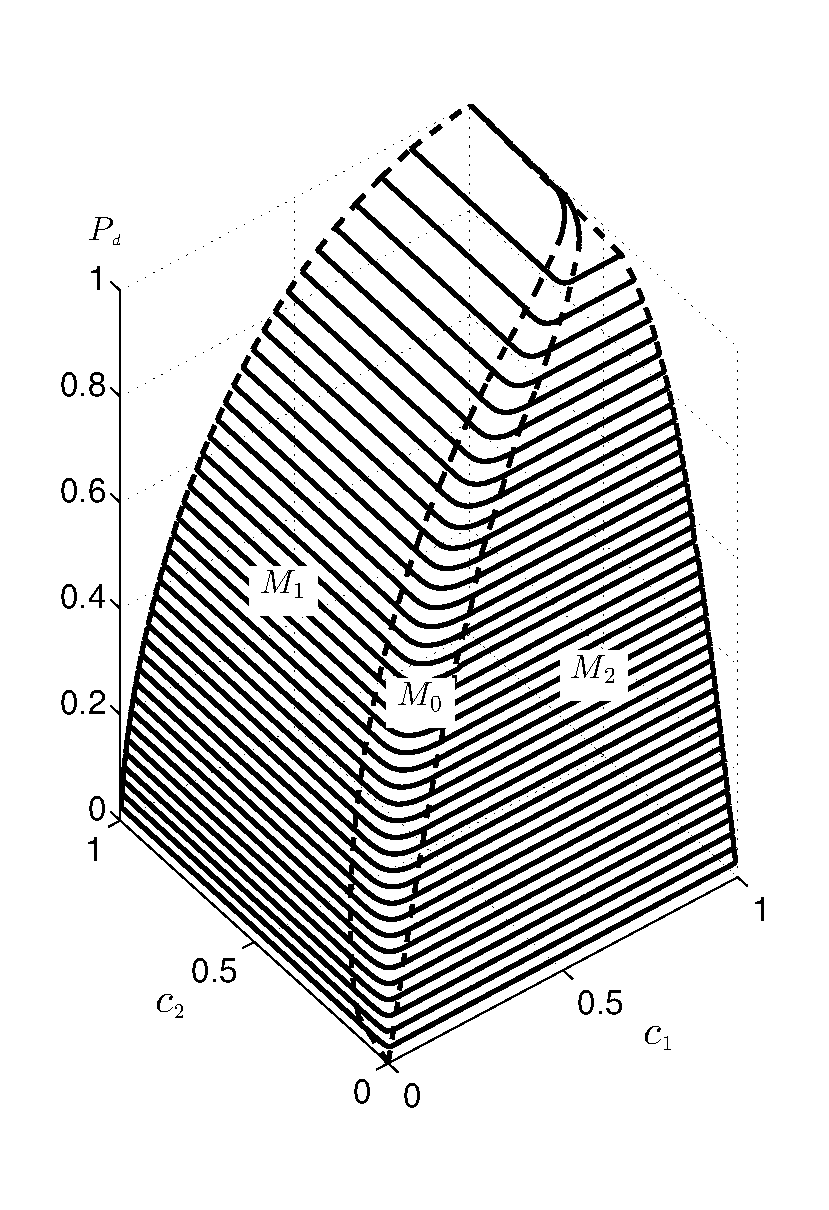
\includegraphics[width=12cm, height=16cm]{3/ROC2.eps}
\caption{The M-ROC surface for Gaussian Hypotheses.}
\label{pic: LJS}
\end{figure}

\noindent \textbf{Example 2:}

Next we consider a more general case of $M+1$ hypotheses given by 
\begin{equation}
\label{equ: m+1 Gaussian Hypo}
\begin{split}
H_0:\;\;\;\;\;\;&X\sim \mathcal{N}(\mu_0, \sigma_0^2)\\
H_1:\;\;\;\;\;\;&X\sim \mathcal{N}(\mu_1, \sigma_1^2)\\
  ......\\
H_M:\;\;\;\;\;\;&X\sim \mathcal{N}(\mu_M, \sigma_M^2)
\end{split}
\end{equation}
We will show when $\sigma_0^2 = \sigma_1^2 = ... = \sigma_M^2$ and $\mu_0 < \mu_i (i = 1, ..., M)$, the region achieved by ENP test with $k_i \geq 0 (i = 1, ..., M)$ degenerates to a curve.

Consider
\begin{equation}
\label{equ: define gx}
g(x) = \sum_{i=1}^{M}k_i\frac{f_i(x)}{f_0(x)}.
\end{equation}
Since 
\begin{equation}
\label{equ: gaussian PDF}
f_i(x) = \frac{1}{\sqrt{2\pi\sigma_i^2}}\exp(-\frac{(x-\mu_i)^2}{2\sigma_i^2}).
\end{equation}
we have
\begin{equation}
\label{g00}
g(x) = \sum_{i=1}^{M}k_i\frac{\frac{1}{\sqrt{2\pi\sigma_i^2}}\exp(-\frac{(x-\mu_i)^2}{2\sigma_i^2})}{\frac{1}{\sqrt{2\pi\sigma_0^2}}\exp(-\frac{(x-\mu_0)^2}{2\sigma_0^2})}
\end{equation}
Substitute  $\sigma_i^2 = \sigma_0^2 (i = 1, ..., M)$ into \eqref{g00}, we have 
\begin{equation}
\label{equ: gx cc}
g(x) = \sum_{i=1}^{M}k_i\exp(\frac{(\mu_i - \mu_0)(2x-\mu_i - \mu_0)}{2\sigma_0^2})
\end{equation}
Defining $p_i = \frac{\mu_i - \mu_0}{2\sigma_0^2}$, \eqref{equ: gx cc} can be written as
\begin{equation}
g(x) = \sum_{i=1}^{M}k_i\exp(p_i(2x-\mu_0 - \mu_i)
\end{equation}
From the condition $\mu_0 < \mu_i (i=1, ..., M)$, we can see $p_i >0$ and  $g(x)$ is a monotonically increasing function with $x$. Here from \textbf{Property 1} we know that $M_0$ (the region achieved by the ENP test with $k_i \geq 0 (i=1, ..., M)$) degenerates to a curve. Moreover, for a specific $\mathbf{c}$, the decision rule is 
\[
x \substack{H_0 \\ \leq \\ > \\ \bar{H}_0} x_0
\]
where $x_0 = \min\{F_1^{-1}(c_1), ..., F_M^{-1}(c_M)\}$. The associated probability of detection is
\[
P_d = F_0(x_0)
\]

Figure \ref{pic: surface for same variance} shows the M-ROC surface for $M=2$, $\mu_0 = 0$, $\mu_1 = 1$, $\mu_2 = 2$ and $\sigma_0^2 = \sigma_1^2 = \sigma_2^2 = 1$. 
Similar to Example 1, the whole M-ROC surface is divided into three regions ($M_1$, $M_0$ and $M_2$) as it is shown in Figure \ref{pic: surface for same variance}.  We have proved, in this example region $M_0$ degenerates to a curve.  
From Figure \ref{pic: surface for same variance}, we know that in region $M_1$, $P_d$ increases if and only if the value of $c_1$ increases, the value of $c_2$ does not affect $P_d$. On the opposite, in region $M_2$, $P_d$ increases if and only if the value of $c_1$ increases, it does not change with $c_2$. In region $M_0$, $P_d$ increases if and only if both $c_1$ and $c_2$ increase (This is different from Example 1, because in this case, region $M_0$ degenerates to a curve). 
In all these three regions, $P_d$ is non-decreasing with respect to $c_1$ and $c_2$. 

From the definition of $M_0$, we know $M_0$ is the region can also be achieved by both ENP test and MENP test. For the rest part of the M-ROC surface, only the MENP test can provide the solution. We can see, comparing to the ENP test, the MENP test has a much larger achievable region (the MENP test can achieve the $P_d$ for the whole $c_1-c_2$ plane, while the ENP test can only achieve the $P_d$ when $(c_1, c_2)$ lies in $\alpha^+$, which is also a curve because $\alpha^+$ is the projection of $M_0$). 

\begin{figure}[!t]
\centering
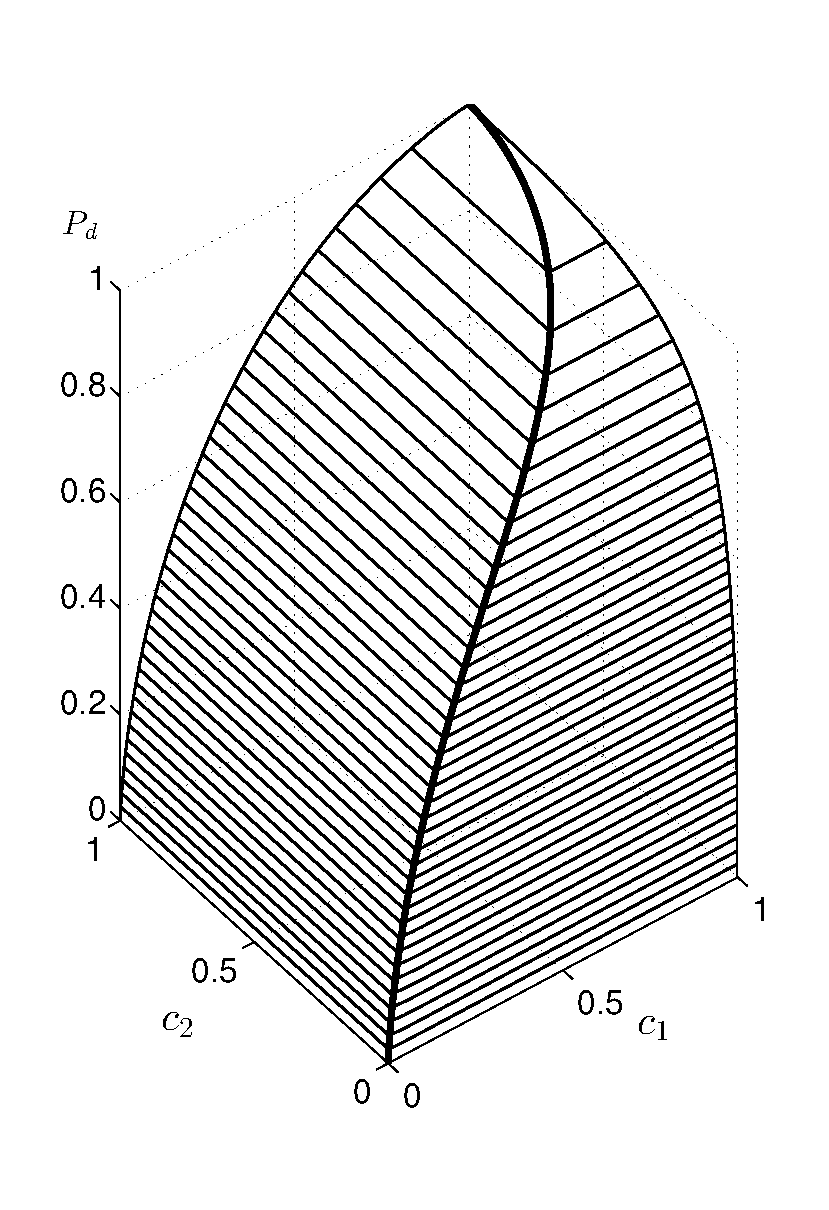
\includegraphics[width=12cm, height=16cm]{3/gaussian.eps}
\caption{The M-ROC for Gaussian distribution with same variance.}
\label{pic: surface for same variance}
\end{figure}
